\documentclass[12pt,a4paper,finnish]{article}

% Jotain paketteja...
\usepackage[finnish]{babel}
\usepackage[T1]{fontenc}
\usepackage[utf8]{inputenc}
\usepackage{url}
\usepackage[nomargin,inline,marginclue,draft]{fixme}
\usepackage{comment}
\usepackage{graphicx}
\usepackage{fullpage}
\usepackage{hyphenat}
\usepackage{minted}
\usepackage{color}
\usepackage{xcolor}

% Tyylejä
\setlength{\parindent}{0mm}
\setlength{\parskip}{3mm plus0.5mm minus0.5mm}

% Kieliä
\newcommand\eng[1]{#1}
\newcommand\eb[1]{\texttt{#1}}

% Otsikko tähän
\title{Otsikko}
\date{\today}
\author{Henrik Lievonen \\ Helsingin matematiikkalukio}

\begin{document}
	% Etusivu
	\begin{titlepage}
	\begin{center}
		\vspace*{\fill}
	
		
\includegraphics[width=0.6\textwidth]{logo}~\\[1cm]
		
		{\huge \bfseries Ohjelmointikieli opetuskäyttöön} \\[0.4cm]
		
		{\Large Henrik Lievonen\\
		Helsingin matematiikkalukio}
		
		{\large Ohjaaja:\\
		Antti Laaksonen\\
		Helsingin yliopisto}
		
		{\large \today}
		
		\vfill		
	\end{center}
\end{titlepage}
	\thispagestyle{empty}

	% Tiivistelmä
	\newpage
	\thispagestyle{empty}
	\section*{Tiivistelmä}
Tässä on tarkoitus tiivistää tutkielman sisältö.
	\newpage

	% Sisällysluettelo	
	\tableofcontents
	\thispagestyle{empty}
	\newpage

	% Sisältö alkaa tästä
	\setcounter{page}{1}
	
	% Täällä lyhyesti tiivistetään raportin sisältö sekä kerrotaan sen taustoista
% Lisäksi täällä kerrotaan myös projektin syntyhistoriasta

\section{Johdanto}
\begin{comment}
Tietokoneet ymmärtävät konekieltä.
Konekieli muodostuu yksinkertaisisista komennoista,
joiden nopeaan suorittamiseen tietokoneet on suunniteltu.
Ihmiset ovat kuitenkin huonoja kirjoittamaan konekieltä
sen alkukantaisten komentojen vuoksi.
Ihmisiä varten onkin kehitelty erilaisia ohjelmointikieliä,
jotka sisältävät erilaisia abstraktioita ohjelmoinnin helpottamiseksi.

Muunnos ohjelmointikielestä konekieleen ei kuitenkaan aina ole yksinkertainen.
Monet ohjelmointikielten abstraktiot voidaan toteuttaa hyvinkin eri tavoin konekielessä,
sillä eri tietokonearkkitehtuurit sisältävät hyvinkin erilaisia konekielisiä komentoja.
Lisäksi lyhyistäkin ohjelmakoodinpätkistä voi syntyä pitkiä konekielisiä ohjelmia,
joten pientenkin ohjelmien muuttaminen konekieleksi voi viedä ohjelmoijalta tunteja.

Tämän prosessin automatisoimiseksi on kehitetty ohjelmia, joita kutsutaan kääntäjiksi.
Kääntäjä on yksinkertaisesti ohjelma, joka muuttaa koodia muodosta toiseen.
Usein tämä tarkoittaa ohjelmointikielen muuttamista konekieleksi,
mutta on myös olemassa kääntäjiä,
jotka kääntävät ohjelmointikieliä toisikseen.
Tällaisia kääntäjiä kutsutaan source-to-source-kääntäjiksi.
\end{comment}

Tässä raportissa kerron kääntäjien toiminnasta yleisesti
sekä itse sunnittelemastani ja toteuttamastani ohjelmointikielestä ja kääntäjästä -- EppaBasicista.

Ohjelmointikielen toteuttamisessa on ollut itseni lisäksi mukana
Sami Kalliomäki (opiskelija, Karkkilan lukio),
joka on suunnitellut ja toteuttanut ohjelmointikielen ympärille tehdyn verkkosivuston
sekä auttanut muutenkin kielen suunnittelussa,
sekä Antti Laaksonen (Helsingin yliopisto),
joka on toiminut vaikuttavana taustavoimana projektin takana.
Lisäksi haluan kiittää kaikkia \#datatahti (IrcNet)- ja \#eppabasic (IrcNet)-kanavien projektiin osallistuineita henkilöitä.

\fxnote{Laajenna johtantoa: Muista basiceista ja niiden historiasta, koodaus peruskoulussa, eb ollut käytössä leireillä}

%Dart
%Codeacatemy
%
%Kopioi tänne githubista historiaa.
	% Täällä kerrotaan aikaisemmista, vastaavista projekteista

\section{Aikaisempia vastaavia ohjelmia}
Monia kieliä on käännetty selainympäristöön (esim. Python, Lua) \cite{repl.it}
\\
Scratch
	\section{EppaBasic-ympäristö}
EppaBasicin tärkein tavoite on olla
helppo oppia,
mutta samalla mahdollistaa
monipuolisten ohjelmien toteuttamisen.
Yksinkertaiset ja helpot grafiikkakomennot ovat tärkeitä,
sillä moni aloitteleva (ja miksei myös kokenutkin)
ohjelmoija haluaa nähdä työnsä tulokset.

Toinen EppaBasicin tärkeä tavoite on,
että se on helppoa ottaa käyttöön.
Usein uutta ohjelmointikieltä käyttöön otettaessa
täytyy ladata ja asentaa useita ohjelmia,
jotka pitää vielä määrittää
toimimaan keskenään.
Monissa kouluissa
ongelmia saattaa lisäksi aiheuttaa byrokratia,
joka vaikeuttaa uusien ohjelmistojen asentamista
koulun tietokoneille.
EppaBasic onkin toteutettu
nettiselaimessa toimivaksi, joten
käyttöönotto onnistuu
helposti koneissa valmiiksi
olevilla ohjelmilla.

Ennen projektin aloittamista pohdimme,
täyttäisikö jokin olemassa oleva
kieli jo nämä tavoitteet.
Kuitenkin miettiessämme vaihtoehtoja
useat kielet olivat vanhentuneita,
niiden asentaminen tai oppiminen on hankalaa,
tai niillä grafiikan tekeminen on työlästä.
Tämän takia päädyimme uuden kielen tekemiseen.
Oman ohjelmointikielten luominen on lisäksi hauskaa
ja opettavaista.

\subsection{Käyttöliittymä}
\begin{figure}[h]
    \centering
    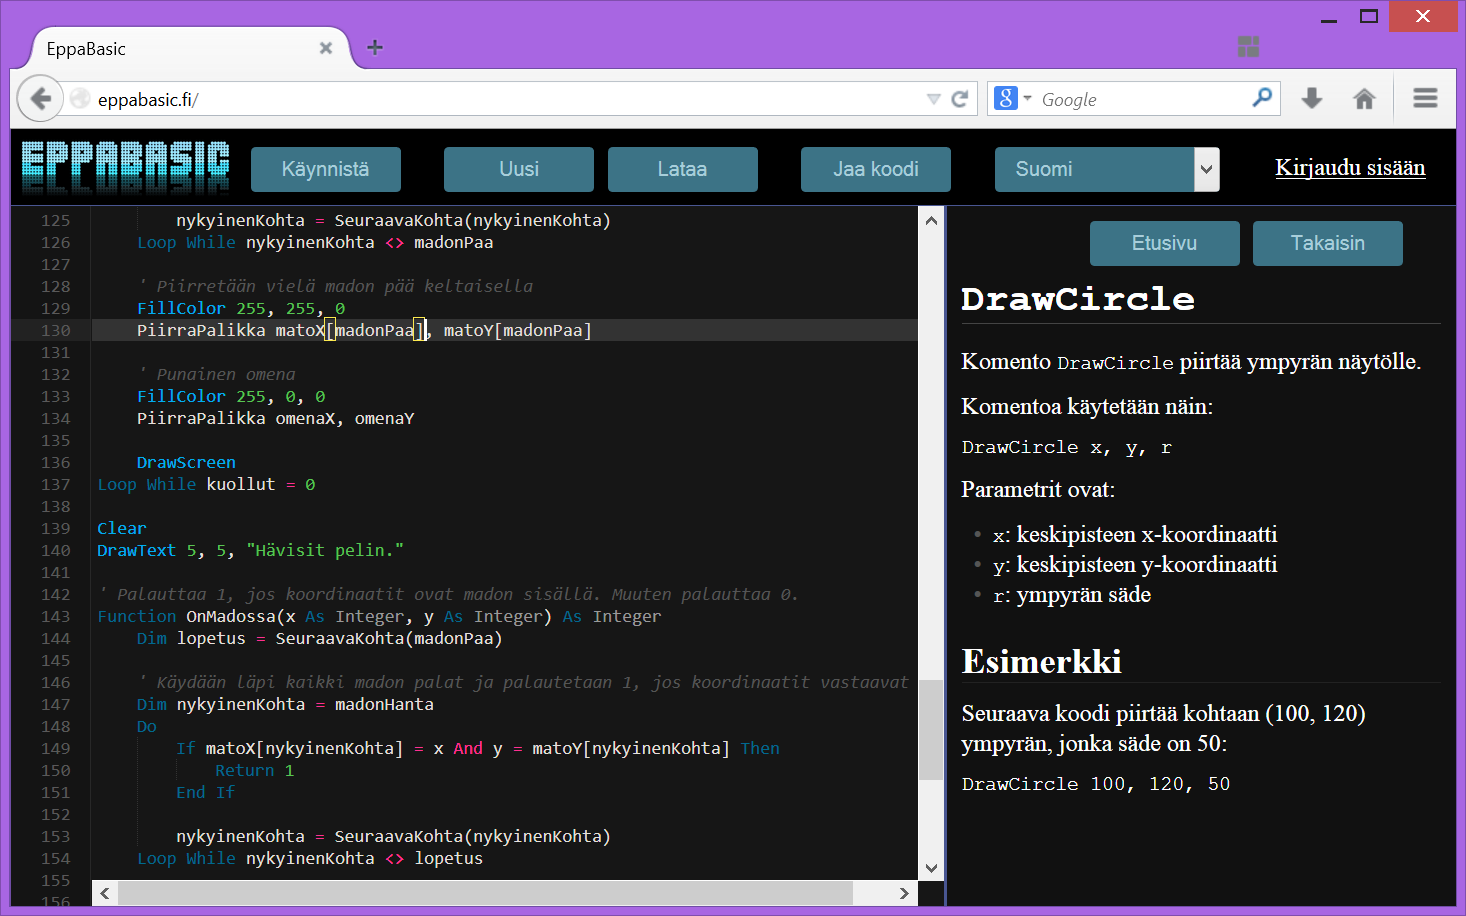
\includegraphics[width=1\textwidth]{kayttoliittyma}
    \caption{EppaBasicin käyttöliittymä. Ylhäällä työkalupalkki, vasemmalla koodimuokkain ja oikealla käyttöohje.}
    \label{img:kayttoliittyma}
\end{figure}

EppaBasicin käyttöliittymä on toteutettu
kokonaan käyttäen HTML:ää ja JavaScriptiä.
Näin on saatu aikaan kaikissa moderneissa
selaimissa toimiva yhtenäinen käyttöliittymä.

EppaBasicin käyttöliittymä tarjoaa kaikki
ohjelmointiin tarvittavat toiminnot.
Yläpalkissa on koodin suorittamisen käynnistävä
nappi sekä napit koodin tallentamiseen ja lataamiseen.
Lisäksi koodin voi jakaa muille käyttäjille linkin avulla.
Kirjautumalla sisään koodin voi tallentaa
omaan hakemistoon, jolloin se on käytettävissä
kaikilla tietokoneilla.

Käyttöliittymän vasemmalla reunalla on
koodimuokkain, johon
ohjelmakoodi kirjoitetaan.
Koodimuokkaimen oikealla puolella on
käyttöohje, jossa on kaikille
EppaBasicin funktioille
ja toiminnoille ohje esimerkkeineen.

EppaBasicin koodimuokkain mahdollistaa
virheiden ilmoittamisen käyttäjälle jo
koodia kirjoitettaessa.
Näin käyttäjä saa heti palautetta tekemistään
virheistä ja voi korjata ne saman tien.
Virhe sisältää käyttäjän oman
kielisen kuvauksen virheestä
(ks. Kuva \ref{img:virhe}).

\begin{figure}[h]
    \centering
    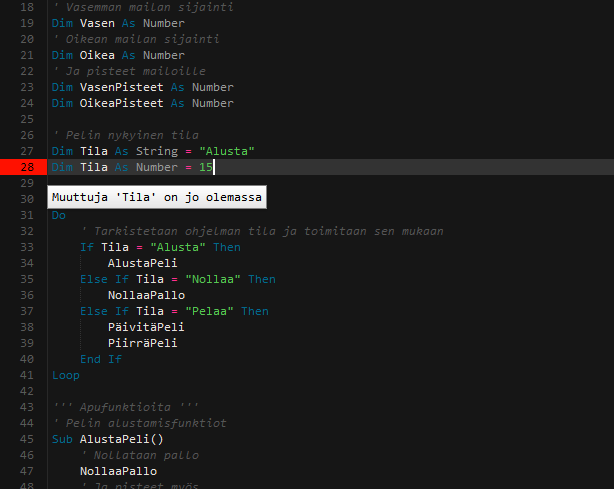
\includegraphics[width=0.5\textwidth]{virhe}
    \caption{EppaBasicin koodimuokkain, jossa näkyy käyttäjän tekemä virhe sekä virheen selitys.}
    \label{img:virhe}
\end{figure}

\subsection{Kieli}
EppaBasicin ohjelmointikieli tukee
muuttujia,
ehto- ja toistorakenteita,
matemaattisten lausekkeiden laskemista,
aliohjelmia, funktioita,
merkkijonoja ja
taulukoita.
EppaBasicissa on myös
laaja standardikirjasto,
jossa on matematiikka-,
merkkijono-, syöte- ja
grafiikkakomentoja.

Koodi \ref{code:geometria} näyttää,
miten EppaBasicilla voi piirtää
yksinkertaisia geometrisia muotoja.
Heittomerkin \eb{'} jälkeinen
teksti rivillä on kommenttia,
jota EppaBasic ei suorita.
Kommentit on tarkoitettu
työkaluksi ohjelmoijalle
koodin selkeyttämiseen.

\codeandimage{geometria}{Geometriaesimerkki}{code:geometria}

EppaBasicissa on
\eb{For}-toistorakenne, jonka
avulla voi suorittaa saman
koodin monta kertaa.
Toistettava koodi alkaa
\eb{For}-avainsanaa seuraavalta
riviltä ja loppuu ennen riviä,
jolla on \eb{Next}-avainsana.
\eb{For}-rakenteen sisällä voi
käyttää toistorakenteessa määriteltyä
muuttujaa, jonka arvo käy läpi
kaikki luvut annetulla välillä
(ks. Koodi \ref{code:for-geometria}).

\codeandimage{for-geometria}{Geometriaa \eb{For}-rakenteella}{code:for-geometria}

\eb{For}-toistorakennetta voi
käyttää myös matemaattisten 
ongelmien ratkausemiseen
(ks. Koodi \ref{code:for-summa}).

\codeandimage{for-summa}{Ohjelma, joka laskee summan $1^2+2^2+3^2+...+100^2$.}{code:for-summa}

EppaBasicilla tehdystä pelistä
esimerkkinä toimii
kielellä tehty moninpelattava
Pong-peli
(ks. Kuva \ref{img:pong}).
Pelin koodi on liitteessä \ref{app:pong}.
Peliä voi kokeilla myös
EppaBasicin sivustolla osoitteessa
\url{http://eppabasic.fi/#PONG}.

\begin{figure}[h]
    \centering
    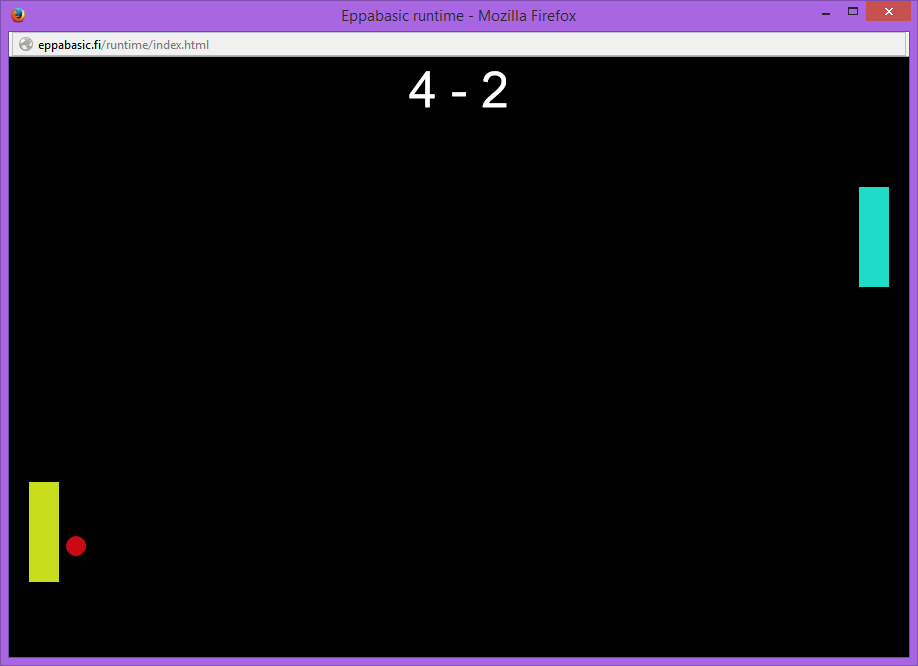
\includegraphics[width=0.5\textwidth]{pong}
    \caption{EppaBasicilla toteutettu kahdenpelattava Pong-peli.}
    \label{img:pong}
\end{figure}
	% Täällä kerrotaan sivuston sekä kääntäjän teknisestä toteutuksesta.

\section{Tekninen toteutus}
Miten toteutettu?

\subsection{Käyttöliittymä}
Tässä kerrotaan käyttöliittymän rakenteesta.
Pääasiassa kerrotaan, että on toteutettu html:llä sekä javascriptillä.
Lisäksi kerrotaan kirjautumismahdollisuudesta sekä
sen tuomista eduista (tallentaminen, jakaminen).
	
\subsection{Kääntäjä}
Kääntäjään todellisesta toteutuksesta olisi tarkoitus kertoa tässä.

\subsection{Ajoympäristö}
Tässä on tarkoitus kertoa uudesta ajoympäristöstä.
Toimii webworkereilla taustasäikeessä.
Suoritusta katkotaan kaksisuuntaisen liikenteen sallimiseksi.
Toiseen suuntaa kulkee grafiikkakomennot ja toiseen suuntaan
käyttäjän syötteet sekä joskus myöhemmin mahdollisesti
myös debug-komennot.
	\section{Yhteenveto}
\fxnote{Kokoa tänne tulevaisuus. Hieman puutteista ja mihin tarkoitukseen kieli on kehitetty. Käännä negatiiviset asiat positiivisiksi: ''Kehitetään toimintavarmuutta'' yms.}

EppaBasic on suomalainen ohjelmointikieli,
jossa on täysin suomenkielinen käyttöliittymä.
Kieli on Basic-kielien tapaan englanninkielinen,
jotta muihin ohjelmointikieliin vaihtaminen
olisi mahdollisimman vaivatonta.
EppaBasicin oppiminen on helppoa
tehokkaan grafiikkamoottorin ja
yksinkertaisten komentojen ansiosta.
Lähitulevaisuudessa EppaBasicista on tarkoitus
saada varteenotettava vaihtoehto niin ohjelmoinnin
kouluopettamiseen kuin itseopiskeluunkin.

Tämän raportin kirjoitushetkellä työn alla
on uuden kääntäjän luominen,
minkä tarkoitus on parantaa kääntäjän
toimintavarmuutta ja käännöksen laatua.
Kehitystietä on valitettavasti hidastanut kehittäjien
lukiopiskelu sekä lähestyviin ylioppilaskokeisiin
valmistautuminen.
	% Täällä listataan raportin teossa käytetyt lähteet

\begin{thebibliography}{99}

\bibitem{repl.it}
	Repl.it-sivusto \url{http://repl.it/languages} (luettu 22.10.2014)

\bibitem{eac2e}
	Keith D. Cooper \& Linda Torczon,
	\emph{Engineering a Compiler}.
	Morgan Kaufmann Publishers,
	Second Edition,
	2012.

\bibitem{basic}
	Thomas E. Kurtz,
	\emph{History of programming languages I}, Osa XI.
	ACM,
	1981.

\bibitem{pascal}
	Niklaus Wirth,
	\emph{The programming language Pascal}.
	Acta informatica,
	1971.
	
\bibitem{language_history}
	A History of Computer Programming Languages \url{http://cs.brown.edu/~adf/programming_languages.html} (luettu 24.1.2015)
	
\bibitem{OPS_2016}
	OPS 2016 - Esi- ja perusopetuksen opetussuunnitelman perusteiden uudistaminen \url{http://www.oph.fi/ops2016} (luettu 27.1.2015)

\bibitem{koodi2016_ops}
	Koodi2016 | Miten OPS muuttuu ja miksi? \url{http://koodi2016.fi/ops.html} (luettu 27.1.2015)

\bibitem{scratch}
	Maloney, John H., et al.,
	Programming by choice: urban youth learning programming with scratch.
	ACM SIGCSE Bulletin,
	2008.

\bibitem{cb}
	CoolBasic - Game Creation \url{http://www.coolbasic.com/index.php?lang=fi} (luettu 30.1.2015)
	
\bibitem{vb.net}
	Visual Basic \url{https://msdn.microsoft.com/en-us/library/2x7h1hfk.aspx
} (luettu 30.1.2015)

\bibitem{bb}
	The Official Blitz Website \url{http://www.blitzbasic.com/} (luettu 1.2.2015)

\bibitem{sb}
	Microsoft Small Basic \url{http://smallbasic.com/} (luettu 1.2.2015)

% HTML&JS
\bibitem{mdn_canvas}
	Canvas - Web API Interfaces | MDN \url{https://developer.mozilla.org/en-US/docs/Web/API/Canvas_API} (luettu 10.11.2014)

\bibitem{mdn_about_js}
	About JavaScript - JavaScript | MDN \url{https://developer.mozilla.org/en-US/docs/Web/JavaScript/About_JavaScript} (luettu 10.11.2014)
	
\bibitem{w3c_html}
	HTML5 \url{http://www.w3.org/TR/html5/} (luettu 10.11.2014)

\bibitem{w3c_web_worker}
	Web Workers \url{http://www.w3.org/TR/workers/} (luettu 14.11.2014)

\bibitem{caniuse_canvas}
	Can I use... Support tables for HTML5, CSS3, etc \url{http://caniuse.com/#feat=canvas} (luettu 19.11.2014)

\bibitem{asm.js}
	asm.js \url{http://asmjs.org/spec/latest/} (luettu 23.1.2015)

% Uutiset
\bibitem{hs_kiuru}
	Ministeri Kiuru: Ohjelmointi peruskoulun opetussuunnitelmaan - Koulu - Kotimaa - Helsingin Sanomat \url{http://www.hs.fi/kotimaa/a1390279526604} (luettu 27.1.2015)
	
\bibitem{hs_eka}
	Ekaluokkalaisten ohjelmointiopetus alkaa vuonna 2016 – Espoon koodikerhosta saa esimakua - Tiede - Helsingin Sanomat \url{http://www.hs.fi/tiede/a1401942756096} (luettu 27.1.2015)

% Komponentit&kirjastot
\bibitem{ace_about}
	Ace - The Highg Performance Code Editor for the Web \url{http://ace.c9.io/} (luettu 11.11.2014)

\bibitem{requirejs}
	RequireJS \url{http://requirejs.org/} (luettu 21.1.2015)
	
\bibitem{r.js}
	jrburke/r.js \url{https://github.com/jrburke/r.js/} (luettu 21.1.2015)
	
\bibitem{jquery}
	jQuery \url{http://jquery.com/} (luettu 21.1.2015)

\bibitem{markdown}
	Daring Fireball: Markdown \url{http://daringfireball.net/projects/markdown/} (luettu 21.1.2015)
	
\bibitem{marked}
	chjj/marked \url{https://github.com/chjj/marked} (luettu 21.1.2015)
	
\bibitem{apache}
	Welcome! - The Apache HTTP Server Project \url{http://httpd.apache.org/} (luettu 1.2.2015)

\bibitem{django}
	The Web framework for perfectionists with deadlines | Django \url{https://www.djangoproject.com/} (luettu 1.2.2015)

\bibitem{postgresql}
	PostgreSQL: The world's most advanced open source database \url{http://www.postgresql.org/} (luettu 1.2.2015)

\end{thebibliography}

		
	
	%% Täällä kerrotaan kielen suunnitettelulähtökohdista
\section{Tavoitteet}
Omalle projektillemme asetimme monia tavoitteita.
Näistä tärkeimpänä voidaan pitää yksinkertaisuutta
sekä matalaa oppimiskäyrää.
Kielellä täytyy myös voida helposti luoda grafiikkaa,
sillä monien aloittelijoiden ohjelmointi-into loppuu siihen,
että graafisesti näyttävien pelien tekeminen ei onnistukaan terminaalissa.

Toinen tärkeä tavoite on,
että kielen käyttöönotto on mahdollisimman helppoa.
Usein uutta ohjelmointikieltä käyttöönottaessa
kuluu tunteja aikaa ohjelmointiympäristön asentamiseen.
Aloittelijoille tämä on usein lannistavaa,
mikä pysäyttää ohjelmointihalut alkumetreilleen.
Halusimme myös, että ohjelmointikieli toimii mahdollisimman monella käyttöjärjestelmällä.

Ennen projektin aloittamista mietimme,
täyttäisikö jokin olemassa oleva kieli jo nämä tavoitteet.
Kuitenkin miettiessämme vaihtoehtoja
olivat useat kielet joko vanhentuneita,
niiden asentaminen tai oppiminen on hankalaa,
tai niillä grafiikan tekeminen on työlästä.
Tämän takia päädyimme uuden kielen tekemiseen.

\begin{comment}
Usein uutta ohjelmointikieltä käyttöönottaessani
minulla kuluu enemmän aikaa ohjelmointiympäristön asentamiseen
kuin uuden kielen oppimiseen.
Vaikka tämä ongelma ei suoranaisesti
\end{comment}

\begin{anfxnote}
Tänne on tarkoitus listata projektin tavoitteita.
\\
Miksi uusi ohjelmointikieli?
\\
Mitä uutta?
\\
Miten erottuu?
\end{anfxnote}		% Toteutukseen
	%% Yleistä höpinää kääntäjien toiminnasta sekä käsitteiden selityksiä

\section{Teoriaa ja määritelmiä}
Kääntäjän toiminta voidaan jakaa pääasiallisesti kolmeen päävaiheeseen:
\eng{front-end}, välivaihe ja \eng{back-end}.
Seuraavaksi selitetään, mitä näillä vaiheilla tarkoitetaan
sekä määritellään muita raportissa käytetäviä käsitteitä.


\subsection{Front-end}
Front-end on kääntämisen ensimmäinen päävaihe.
Se lukee käyttäjän kirjoittaman lähdekoodin
ja muuttaa sen kääntäjän sisäiseen muotoon.
Front-end on ainoa osa, joka käsittelee ohjelmaa kokonaisuutena
ja tietää ohjelmointikielen syntaksin.
Muut vaiheet eivät välttämättä ole riippuvaisia käännettävästä
kielestä vaan voivat toimia front-endistä riippumatta.
Front-endin tehtäviin kuuluu myös käännöksen aikaisista virheistä tiedottaminen.

\subsection{Välivaihe}
Välivaihe on kääntämisen toinen päävaihe.
Sen tarkoitus on muokata ohjelmaa jollakin tavalla paremmaksi.
Yksinkertaisimmillaan välivaihe vain muuttaa ohjelman sisäisestä
muodosta toiseen.
Useissa kääntäjissä on monia välivaiheita, joita saatetaan jopa
iteroida useita kertoja paremman lopputuloksen saamiseksi.
Paremmalle ei tässä yhteydessä ole yksikäsitteistä määritelmää,
vaan se saattaa eri yhteyksissä tarkoittaa esimerkiksi
nopeampaa suoritusta, pienempää käännetyn ohjelman kokoa
tai pienempää muistinkäyttöä. Useimmiten suorituksen nopeuttaminen
on pääintressi tietokoneohjelmissa, kun taas muistin käytön
vähentäminen on tärkeää sulautetuissa järjestelmissä.
Täälaista ohjelmakoodin parantamista kutstuaan optimoimiseksi,
ja vastaavasti sitä tekeviä välivaiheta optimoijiksi.

\subsection{Back-end}
\eng{Back-end} on kääntämisen viimeinen vaihe.
Sen tehtävä on muutta ohjelmakoodi lopulliseen muotoonsta,
jota suorittamiseen käytetty ympäristö ymmärtää.
Ajoympäristö on usein joko suoraan rautatason laite
tai virtuaalikone, joka ajon aikana muuttaa koodin raudan ymmärtämään muotoon
tai vaihtoehtoisesti tulkitsee koodia.
\eng{Back-end} on periaatteessa kääntämisen ainoa vaihe,
joka välittää käännöksen kohteen arkkitehtuurista,
tosin joskus myös viimeiset välivaiheen vaiheet riippuvat kohdearkkitehtuurista.

\subsection{Syntaksi}
Syntaksi tarkoittaa kielen kielioppia.
Ohjelmoidessa sen on tarkoitus olla täysin yksiselitteinen,
jottei kääntäjän tarvitse arvuutella,
mitä ohjelmoija haluaa ohjelman tekevän.
Syntaksi esimerkiksi määrittelee,
että $If$-avainsanaa on seurattava $Boolean$-tyypiksi evaluoituva lauseke
tai mitkä nimet ovat sallittuja muuttujannimiä.

\subsection{Lähdekoodi}
Lähdekoodi on käyttäjän kirjoittama kuvaus ohjelman toiminnasta.
Kääntäjä muuttaa lähdekoodin kohdekoodiksi,
jota tietokone, virtuaalikone tai tulkki suorittaa.
Lähdekoodi on usein ihmisen helposti ymmärrettävissä
sekä sisältää monia ymmärtämistä helpottavia abstraktioita,
kuten esimerkiksi muuttujat ja komentorakenteet.
Lähdekoodi noudattaa syntaksia.

\subsection{Ohjelmointikieli}
Ohjelmointikieli on syntaksin määrittämä kokonnaisuus.
Ohjelmointikielet voidaan luonnollisten kielien
(suomi, ruotsi, yms.)
tavoin jakaa kielisukuihin,
usein suvun ensimmäisen kielen mukaan.
Ohjelmointikielisukuja ovat esimerkiksi
C-pohjaiset ja
Basic-kielet.
		% -||-
	%\section{Tulevaisuus}
EppaBasicin kehitystä on tarkoitus
jatkaa myös tulevaisuudessa.
Tämän raportin kirjoitushetkellä työn alla
on uusi kääntäjä,
jonka tarkoitus on parantaa käännöksen laatua.
Myöhemmin on lisäksi tarkoitus lisätä
mahdollisuus piirtää bittikarttakuvia
ja toistaa ääntä.
Lähitulevaisuudessa EppaBasicista on tarkoitus
saada varteenotettava vaihtoehto niin ohjelmoinnin
kouluopettamiseen kuin itseopiskeluunkin.
Kehitystietä on valitettavasti hidastanut kehittäjien
lukio-opiskelu sekä lähestyviin ylioppilaskokeisiin
valmistautuminen.

EppaBasicia on tarkoitus käyttää keväällä
ja kesällä 2015 ainakin kahdella kurssilla:
Keväällä Helsingin luonnontiedelukiossa
järjestetään ohjelmoinnin peruskurssi,
joka opetetaan kokonaisuudessaan
EppaBasicilla.
Kesällä kieltä käytetään jälleeen
Helsingin yliopiston LUMA-keskuksen
''Bittejä ja algoritmeja'' -leirillä.	% Yhteenvetoon
	%% Tänne kerätään lopuksi mielipiteitä toteutuksen onnistuneisuudesta

\section{Johtopäätöksiä}
% Miten onnistuttu tavoitteissa?

	% -||-
	
\end{document}
